% source: 论文起草.md L479-L859
\subsection{第二问：弹性分布式算力网络的替代效益与边界}\label{sec:q2}

\textbf{分布式算力网络}是一个随现代互联网发展，人们对计算需求的增加，尤其是近年AI训练与推理需求的增加而出现并兴起的概念。早期最有代表性的构想与实践之一是1995年的\textbf{SETI@home项目\cite{q2cref01}。}

其核心在于将地理上互相分离、已经存在、分属不同机构或个人的计算机连接起来，共享昂贵算力，利用闲置容量，处理单个中心难以独自承担的数据量，并让不同地区的使用者参与。在题目探讨背景下，具体而言，它带来了一种分摊环境压力，使资源条件脆弱的社区也能获得充足算力的方案。

因此，我们希望能够建立这一替代模式的模型，评估它相较于集中式数据中心可能带来的不同维度下的额外效益或者损失。

\subsubsection{分布式算力网络模式}\label{sec:q2-network}

分布式算力网络的硬件根基仍然是算力设施。各算力设施在得到信息任务分配后完成计算，随后通过网络联络交换任务与输出。因此，对于网络中的单个节点，我们依旧以集中式数据中心的性质描述它。

\begin{asum}\label{asum:node}
单体小园区即单个小规模集中式数据中心，各自拥有独立地理条件与建设运营方案，包括分配到的IT功率，发电功率配比，发电方式，建筑布局等。在计算时，这些条件输入第1问所建的集中式数据中心模型。
\end{asum}

网络联络所带来的额外能源消耗以及算力的损失取决于调度方式，算力任务与地区访问次数等众多因素\cite{q2cref03,q2cref02}，全部建模极为困难，因此我们考察其中影响较为显著者：

考虑到小园区自身设施配置限制与园区间联络成本，其具有特点：

年度PUE高于大型园区，通常在1.5以上，表征其需要花费更多电力在设施运维与通讯联络上

$a_s$大于大型园区，表征其IT设施密度较低

考虑评估分布式算力网络造成的资源压力。分布式算力网络中各节点的一大显著特征就是地理上的分散性，从而实现了资源压力的分摊。为了考察这一效应带来的影响，不妨假设：

\begin{asum}\label{asum:no-overlap}
各单体数据中心所用资源互不重叠
\end{asum}

\subsubsection{环境足迹}\label{sec:q2-footprint}

\textbf{根据联合国大学水、环境与健康研究所的探讨与报告，}AI 的环境成本不仅取决于电力使用，更在于对土地和水资源的占用\cite{q2ref01}。电力使用带来的环境成本则主要源于发电过程产生的温室气体排放，部分能源生产过程的用水以及发电设施占地（本文讨论中合并到信息设施土地占用下）

基于这一报告，在题目讨论框架下，我们认为AI数据中心产生的\textbf{环境足迹要素主要}包含\textbf{碳足迹，水足迹，以及土地足迹}。我们比较总算力需求给定情况下不同方案\textbf{运行时}环境足迹的多少，分别对应以下三个量：

$C_{out}$代表给定算力需求下\textbf{单位时间内}产生的碳足迹后文cout表示总量，没有除以时间

$W_{out}$为给定算力需求下\textbf{单位时间内}产生的水足迹

$A_{out}$为给定算力需求下产生的土地足迹

对于给定算力需求$O_{ut}$，由Epoch AI提供的数据可知，对于现有算力设施，能量消耗与算力需求大致呈线性关系。

\begin{figure}[H]
\centering
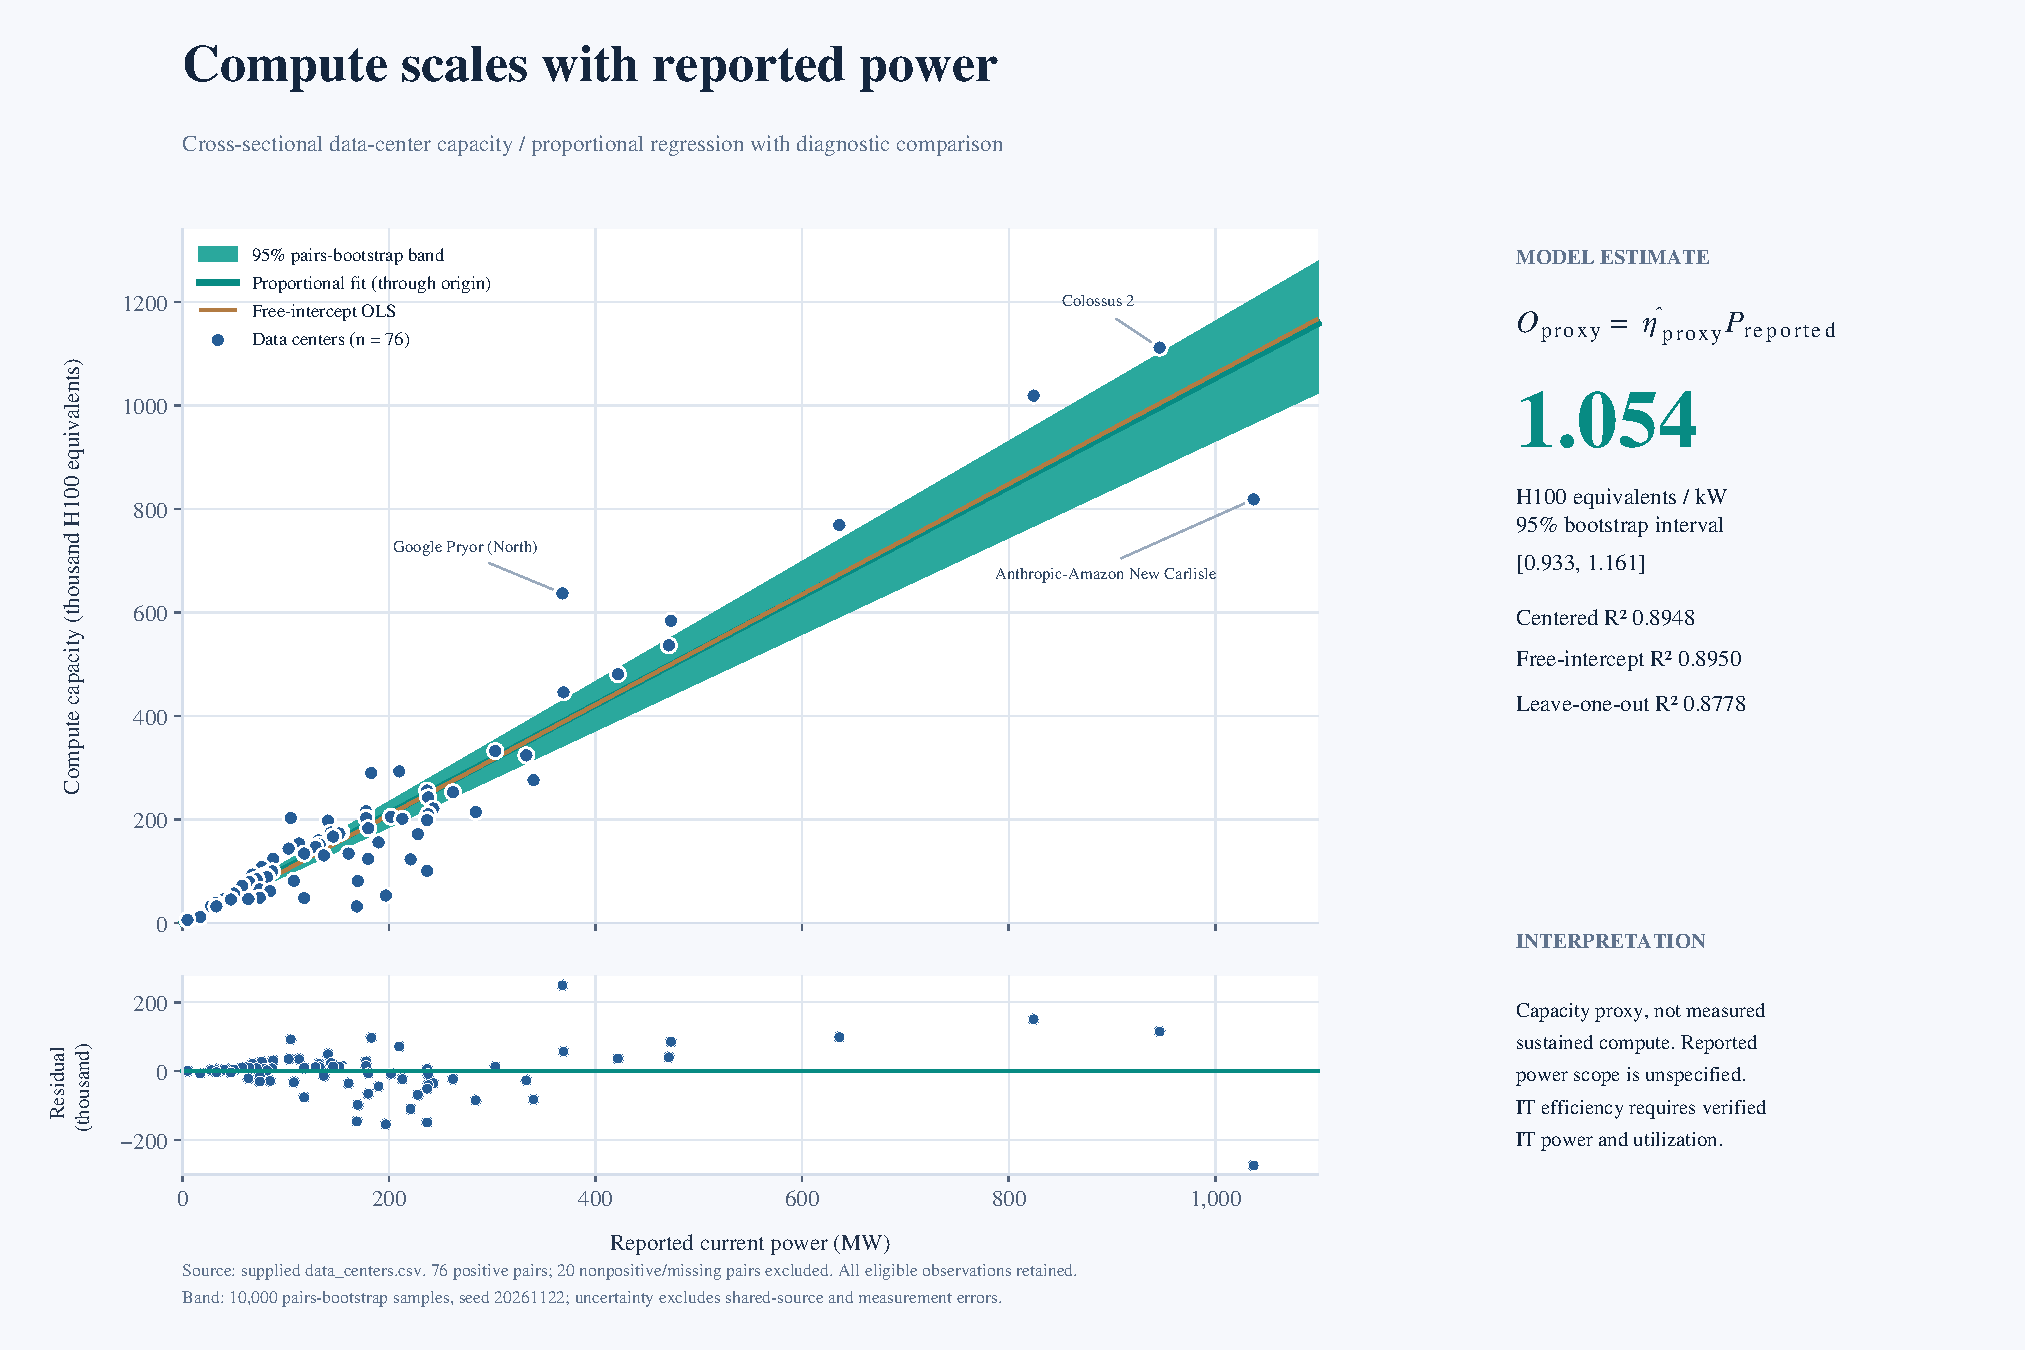
\includegraphics[width=0.72\textwidth]{figures/compute_power_fit.pdf}
\end{figure}

由数据进行过原点最小二乘拟合，得到$\eta_{proxy}=1.0538$，单位H100-equivalent/kW。

$R^2=0.8948$，说明算力大小与报告的IT容量在样本内具有较强的近似比例关系。

因此，对于给定算力要求，可以大致对应其所需的IT容量：

\begin{equation}\label{eq:q2-pit}
P_{\text{IT}}=\frac{O_{ut}}{\eta}
\end{equation}

其中 $O_{ut}$ 是持续提供的算力，$\eta$ 是单位 IT 功率对应的算力。以下统一令 $P_{\mathrm{IT}}$ 的单位为 \textbf{kW}。后文式子用的是MW还是kW

\begin{noteblock}
我们假设的时间尺度下，$\eta$是定值，黄仁勋重新当上英伟达CEO前不太会变
\end{noteblock}

对于每一种资源限制，按照$P_{\mathrm{IT}}$强度反推出对应的足迹或对当地资源的压力。

\paragraph{集中式数据设施}\label{sec:q2-cen}

\subhead{碳足迹}

\textbf{1　核算边界与近似假设}

本文以运行用电相关的二氧化碳排放量表征数据设施的碳足迹。考虑到运行阶段温室气体排放以 CO$_2$ 为主，为降低模型复杂度，采用 CO$_2$ 排放因子，不单独核算 CH$_4$、N$_2$O 等其他温室气体，也不计入燃料开采与运输、设备制造等环节的排放。因此，本文的“碳足迹”仅指上述边界内的运行用电相关 CO$_2$ 排放。

统计期划分为若干运行时段。保留时段是为了描述用电及供电来源的变化，并累计排放。设施用电包含 IT 设备、冷却及配电等，站外广域网用电计入系数k计算。

\textbf{2　计算步骤}

所有功率均指实际运行功率或时段平均功率。电量 E 为功率乘以时段长度所得的中间计算量，单位 MWh。

\textbf{第一步：确定园区设施用电功率}

对于碳足迹，分布式模型沿用集中式模型的设施用电核算方法。新增网络传输等损耗，非线性增长，需根据设施规模估算，此处计入系数k计算。

\begin{equation}\label{eq:q2-facility}
P_{\text{设施},t}=k_tP_{\mathrm{IT},t}
\end{equation}

设施倍率 $k_t$ 将 IT 功率换算为包含冷却、供配电等辅助用电的设施总功率。可近似等于PUE。

\textbf{第二步：区分电网供电与自发电}

在无储能的情景下，各时段满足：

\begin{equation}\label{eq:q2-balance}
P_{\text{电网},t}
+\sum_mP_{\text{自发电},m,t}
=P_{\text{设施},t}.
\end{equation}

电网与自发电的份额由前述供电分配模型确定，并满足电网额度及电源出力限制。式~\eqref{eq:q2-balance} 本身只规定供需平衡，不唯一决定各电源的份额。

\textbf{第三步：将功率换算为电量}

\begin{equation}\label{eq:q2-energy}
\begin{aligned}
E_{\text{电网},t} &= P_{\text{电网},t}\Delta t,\\
E_{\text{自发电},m,t} &= P_{\text{自发电},m,t}\Delta t.
\end{aligned}
\end{equation}

功率单位 MW 乘以时长单位 h，得到电量单位 MWh。

\textbf{第四步：计算并累加各时段排放}

\begin{equation}\label{eq:q2-carbon}
C_{out}{\mathrm{}}
=\sum_t\left[
P_{\text{电网},t}f_{\text{电网},t}
+\sum_mP_{\text{自发电},m,t}f_{\text{自发电},m,t}
\right]\Delta t.
\end{equation}

各来源电量分别乘以对应排放因子，再将所有时段的排放相加，得到 $C_{\mathrm{out}}$，单位为 t CO$_2$。

\textbf{3　官方因子取值及简化公式}

采用中国全国平均电网数据进行近似时，取：

\begin{equation}\label{eq:q2-fgrid}
f_{\text{电网},t}=0.5306\ \mathrm{t\ CO_2/MWh}.
\end{equation}

当自发电全部采用化石能源混合平均情景时，取：

\begin{equation}\label{eq:q2-fself}
f_{\text{自发电},t}\approx0.8273\ \mathrm{t\ CO_2/MWh}.
\end{equation}

采用中国全国平均数据进行近似时，电网因子取 2023 年全国电力平均二氧化碳排放因子；自发电采用 2023 年全国化石能源电力二氧化碳排放因子。数据发布于 2025 年 12 月 31 日\cite{q2bref01,q2bref02}。在缺少最新数据的情况下将上述历史数据作为近似，并在各运行时段保持不变。

风电、光伏在本文发电运行边界内，CO$_2$ 排放近似取零。

\subhead{水足迹}

\begin{equation}\label{eq:q2-qfield}
Q_{\text{现场}} =\mathrm{WUE}\,P_{\mathrm{IT}}
\end{equation}

其中$Q_{\text{现场}}$ 为数据中心正常运营所需的现场耗水流量，包括冷却及辅助设施耗水，不含供电过程的间接耗水。

另外考虑自发电情形产生的耗水：

\begin{equation}\label{eq:q2-qgen}
Q_{\text{发电耗水}}=24\sum_i c_i\bar P_i
\end{equation}

则数据中心总耗水流量为正常运营流量与发电耗水流量之和，即数据中心水足迹$W_{out}$：

\begin{equation}\label{eq:q2-wout}
W_{out}=Q_{\mathrm{DC}}=Q_{\text{现场}}+Q_{\text{发电耗水}}
\end{equation}

\subhead{土地足迹}

在给定功率计划下，按照上文定义以及取值方法，可计算得总需地：

\begin{equation}\label{eq:q2-areq}
A_{\mathrm{req}}=A_{0}+A_{e}+a_sP_{\mathrm{IT}}
\end{equation}

\paragraph{分布式数据设施}\label{sec:q2-dis}

达到给定算力需求的分布式方案，其额外消耗主要来自通讯成本与设备异质性的兼容问题等，主要造成电资源的消耗，在上文已涵盖入模型的电资源压力计算。考虑到因素众多，在此我们做出算力需求可以线性分配到各分布园区的假设。

\begin{asum}\label{asum:no-decay}
算力需求不随分配到各园区而衰减
\end{asum}

将总算力需求分散到各个小园区，有：

\begin{equation}\label{eq:q2-sum-o}
\sum O_{i}=O_{ut}
\end{equation}

随后对于每个小园区，按照独立集中式园区模型，与上同理计算出C，W，和L

最后将每个园区C,W,A求和得到总足迹：

\begin{equation}\label{eq:q2-cout}
C_{out} = \sum C_i
\end{equation}

\begin{equation}\label{eq:q2-wout-sum}
W_{out} = \sum W_i
\end{equation}

\begin{equation}\label{eq:q2-aout}
A_{out} = \sum A_i
\end{equation}

\subsubsection{资源压力}\label{sec:q2-pressure}

对于给定的地理条件，由第一问假设，该地区资源存在一个确定的供给上限，当数据中心消耗资源逼近上限时会对当地资源产生巨大压力。

（美国中期选举的例子）

为表征这种资源压力，我们依次计算数据中心使用资源在当地总剩余可调配资源中的占比。

\paragraph{集中式数据设施}\label{sec:q2-p-cen}

\subhead{水资源压力}

为评估数据中心实际运行对当地造成的\textbf{水资源压力}，考虑到生态基流与已有社会经济用水具有优先保障权，新增项目带来的压力本质上取决于其对河流剩余水资源的消耗程度。因此，我们采用数据中心实际总耗水流量 $Q_{\mathrm{DC}}$ 与第一问所求得的河流剩余可用水量 $Q_{\text{可用}}$ 之比来定义数据中心的\textbf{水资源压力} $R_{\mathrm{W}}$：

\begin{equation}\label{eq:q2-rw}
R_{\mathrm{W}} = \frac{Q_{\mathrm{DC}}}{Q_{\text{可用}}} = \frac{Q_{\mathrm{DC}}}{Q_{\text{河流}} - Q_{\text{生态}} - Q_{\text{其他耗水}}}
\end{equation}

其中，分母 $Q_{\text{可用}} = Q_{\text{河流}} - Q_{\text{生态}} - Q_{\text{其他耗水}}$ 即为第一问中扣除生态保留水量与已有用户取水量后，河段尚可额外分配的剩余可用水量。$R_{\mathrm{W}}$ 直观反映了数据中心对本地剩余水资源空间的占用水平：

\begin{itemize}
\item 当 $R_{\mathrm{W}} \ll 1$ 时，表明数据中心仅消耗了少量剩余可用水量，造成的\textbf{水资源压力}较低，对当地原有供水格局及抗旱缓冲能力影响有限；
\item 当 $R_{\mathrm{W}}$ 趋近于 $1$ 时，说明数据中心几乎耗尽了河流的全部剩余可用水量，意味着当地\textbf{水资源压力}已处于极高水平，水资源竞争激烈且项目抗风险能力较弱。
\end{itemize}

\subhead{电资源压力}

\textbf{确定当地电网剩余可供功率}

\begin{equation}\label{eq:q2-reserve}
P_{\text{余量}}
=P_{\text{项目购电}}-P_{\text{其他负荷}}.
\end{equation}

\textbf{确定项目实际购电功率}

园区在设计工况下的实际购电功率记为 $P_{\text{项目购电}}$，直接采用前述供电分配模型的结果。

\textbf{计算集中式电力资源压力}

\begin{equation}\label{eq:q2-re}
R_{\mathrm{E}}
=\frac{P_{\text{项目购电}}}{P_{\text{余量}}}.
\end{equation}

\subhead{土地资源压力}

由上文算得需地，结合选定地图中的地块，按照上文选择标准得到候选场址的 $A_{\mathrm{eff}}$，即可调配的土地资源面积。随后计算可得土地资源压力，即用地在调配的土地资源的占比：

\begin{equation}\label{eq:q2-ra}
R_A=\frac{A_{\mathrm{req}}}{A_\mathrm{eff}}
\end{equation}

\paragraph{分布式数据设施}\label{sec:q2-p-dis}

继承上文对分布式数据设施假设，我们同理将其按单个集中式中心处理，特别地：

\begin{asum}\label{asum:no-cross}
各分算力中心资源占用无交叉
\end{asum}

计算每个算力中心对\textbf{当地}资源的资源消耗以及当地可用资源，得到各自的各项资源占用率$R$。为衡量总体压力表现，我们\textbf{以最紧张节点作为压力指标：}

\begin{equation}\label{eq:q2-rwmax}
R_W=\max R_i^W,
\end{equation}

\begin{equation}\label{eq:q2-remax}
R_E=\max R_i^E,
\end{equation}

\begin{equation}\label{eq:q2-ramax}
R_A=\max R_i^A,
\end{equation}

\subsubsection{综合评价}\label{sec:q2-eval}

\subhead{环境足迹}

对于\textbf{环境足迹}维度，我们取定该算力规模下的基准环境足 $C_{\mathrm{ref}},W_{\mathrm{ref}},A_{\mathrm{ref}}$（可直接取集中式方案足迹作为基准），以将这三个足迹指标转化为可比较的无量纲指标。

赋予三者权重$w_C,w_W,w_A$并加和。

考虑到资源使用量的绝对量级：10吨相对于1吨碳排放，100吨相对于10吨碳排放，这两次比较从绝对量级的角度而言，后者差异显著更大，但从横向比较的角度而言这种差异是一致的。我们希望比较方案间相对的增长，为了避免绝对量级对评价造成的影响，我们选择再加一层对数抹除绝对量级。

最终得到综合环境足迹指数$F$：

\begin{equation}\label{eq:q2-findex}
F=\ln (w_C\frac{C}C_{\mathrm{ref}}+w_W\frac{W}W_{\mathrm{ref}}+w_A\frac{A}A_{\mathrm{ref}}), \qquad w_C+w_W+w_A=1
\end{equation}

若以集中式方案作为基准方案，即取$C_{\mathrm{ref}}=C_{cen},W_{\mathrm{ref}}=W_{cen},A_{\mathrm{ref}}=A_{cen}$有

\begin{equation}\label{eq:q2-fcen}
F_{cen}=0
\end{equation}

\subhead{资源压力}

对于\textbf{资源压力}维度，我们希望构建惩罚项，使得资源在迫近当地资源上限时有显著的边际效应。

因此，我们先构建压力函数：

\begin{equation}\label{eq:q2-phi}
\phi(R)=\frac{R}{1-R}
\end{equation}

它具有性质：

\begin{equation}\label{eq:q2-phi-prop}
\phi(0)=0, \qquad \lim_{R\to1^-}\phi(R)=+\infty,
\end{equation}

并且其边际效应为：

\begin{equation}\label{eq:q2-phi-deriv}
\frac{\mathrm d\phi}{\mathrm dR} = \frac{1}{(1-R)^2}.
\end{equation}

因此，资源占比较小时增长影响有限，但接近极限时会受到强烈惩罚。

例如：

\begin{equation}\label{eq:q2-examples}
\phi(0.5)=1,\qquad \phi(0.9)=9,\qquad \phi(0.99)=99.
\end{equation}

这正好表达“当地资源接近耗尽时，新增消耗的环境代价快速上升”。

如果任何一项资源达到或超过当地可用上限，直接规定：

\begin{equation}\label{eq:q2-infeasible}
R_k\ge 1 \quad\Longrightarrow\quad \phi=+\infty,
\end{equation}

也就是方案不可行。

为综合三项压力表现，我们赋予三者权重$m_W,m_E,m_A$，得压力表现加权平均值$S$:

\begin{equation}\label{eq:q2-sweighted}
S=m_W\phi(R_W)+m_E\phi(R_E)+m_A\phi(R_A), \qquad m_W+m_E+m_A=1
\end{equation}

\subhead{最终评价}

我们的终极目标是比较集中与分布式方案在\textbf{降低环境足迹和资源压力}这两方面的综合优劣。二者往往不可得兼：分布式算力中心能分摊对当地资源的压力，但同时也可能需要更多资源来代偿设施不集中带来的效率折损问题。

因此，我们最后的评价兼并二者。为比较同等算力任务下集中式与分布式方案在\textbf{环境足迹与资源压力}这两个评价向度下的综合表现，构造综合得分：

\begin{equation}\label{eq:q2-final}
\Omega = F + \lambda S
\end{equation}

$\Omega$反映该方案的环境足迹与资源压力的综合评价：$\Omega$越大，说明该方案环境足迹更严重或对当地资源挤压更严重。$\lambda$表示S项的权重，实际应按F可能的大小差异估计调整。

分别代入两个方案，

$\Omega_{cen}<\Omega_{dis}$说明集中式方案更具优势，反之说明分布式方案更具优势。

